\documentclass[border=2pt]{standalone}
\usepackage{pgfplots}
\begin{document}
    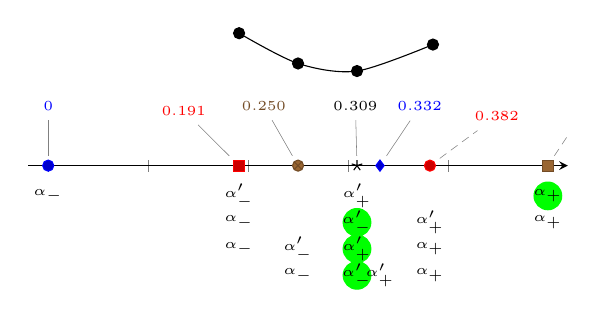
\begin{tikzpicture}
        \begin{axis}[
            % center the x axis
            axis x line=middle,
            % we don't need a y axis line ...
            axis y line=none,
            % ... and thus there is no need for much `height' of the axis
            height=150pt,
            % but `height' also changes `width' which is restored here
            width=\axisdefaultwidth,
            xmin=-0.02,
            xmax=0.52,
            xticklabels={,,}
        ]
         	\addplot coordinates {(0, 0)} node[pin=90:{\tiny $0$}]{};
            \addplot coordinates {(0.191, 0)} node[pin=120:{\tiny $0.191$}]{};
            \addplot coordinates {(0.250, 0)} node[pin=93:{\tiny $0.250$}]{};
            \addplot coordinates {(0.309, 0)} node[pin=92:{\tiny $0.309$}]{};
            \addplot coordinates {(0.332, 0)} node[pin=80:{\tiny $0.332$}]{};
            \addplot coordinates {(0.382, 0)} node[pin=45:{\tiny $0.382$}]{};
            \addplot coordinates {(0.5, 0)} node[pin=70:{\tiny $0.5$}]{};
            
            \addplot[smooth, mark=*] coordinates {(0.191, 3.5) (0.25, 2.7) (0.309, 2.5) (0.385, 3.2) };
            
            \addplot[mark=*, fill=green, draw=green, mark size=5] coordinates {(0.5, -.8)};
            \addplot[mark=text, text mark={\tiny $\alpha_+$}] coordinates {(0.5, -.8)};
            \addplot[mark=text, text mark={\tiny $\alpha'_+$}] coordinates {(0.309, -.8)};
            \addplot[mark=text, text mark={\tiny $\alpha'_-$}] coordinates {(0.191, -.8)};
            \addplot[mark=text, text mark={\tiny $\alpha_-$}] coordinates {(0, -.8)};
            
            \addplot[mark=*, fill=green, draw=green, mark size=5] coordinates {(0.309, -1.5)};
            \addplot[mark=text, text mark={\tiny $\alpha_+$}] coordinates {(0.5, -1.5)};
            \addplot[mark=text, text mark={\tiny $\alpha'_-$}] coordinates {(0.309, -1.5)};
            \addplot[mark=text, text mark={\tiny $\alpha_-$}] coordinates {(0.191, -1.5)};
            \addplot[mark=text, text mark={\tiny $\alpha'_+$}] coordinates {(0.382, -1.5)};
            
            \addplot[mark=*, fill=green, draw=green, mark size=5] coordinates {(0.309, -2.2)};
            \addplot[mark=text, text mark={\tiny $\alpha'_-$}] coordinates {(0.25, -2.2)};
            \addplot[mark=text, text mark={\tiny $\alpha'_+$}] coordinates {(0.309, -2.2)};
            \addplot[mark=text, text mark={\tiny $\alpha_-$}] coordinates {(0.191, -2.2)};
            \addplot[mark=text, text mark={\tiny $\alpha_+$}] coordinates {(0.382, -2.2)};
            
            \addplot[mark=*, fill=green, draw=green, mark size=5] coordinates {(0.309, -2.9)};
            \addplot[mark=text, text mark={\tiny $\alpha_-$}] coordinates {(0.25, -2.9)};
            \addplot[mark=text, text mark={\tiny $\alpha'_-$}] coordinates {(0.309, -2.9)};
            \addplot[mark=text, text mark={\tiny $\alpha'_+$}] coordinates {(0.332, -2.9)};
            \addplot[mark=text, text mark={\tiny $\alpha_+$}] coordinates {(0.382, -2.9)};
            
        \end{axis}
    \end{tikzpicture}
\end{document}